\documentclass[aspectratio=169]{beamer}
\usepackage[utf8]{luainputenc}
\usepackage{amssymb,amsmath}
\usepackage{graphicx}
\usepackage{tikz}
\usepackage{beamercolorthemetud}
\usepackage[backend=biber]{biblatex}
\usepackage{caption}
\captionsetup[figure]{font=scriptsize}
\usepackage{hyperref}

\usepackage{subcaption}
\usepackage[absolute,overlay]{textpos}
  \setlength{\TPHorizModule}{1mm}
  \setlength{\TPVertModule}{1mm}




\addbibresource{bibl.bib}
\setbeamertemplate{bibliography item}{\insertbiblabel}
\usepackage[english]{babel}
\usetheme[]{tud}
\setbeamercolor{background canvas}{bg=}
\setbeamerfont{frametitle}{size=\Large}
\input{macros}



\title{App Idea Presentation: MeetForSport}
\author{Mattis Lahr, Felix Fischer}
\date{19.11.2021}

\einrichtung{\hspace{-1pt}Institute of Systems Architecture}
\datecity{Dresden}




\AtBeginSection[]{\partpage{\usebeamertemplate***{part page}}}
\begin{document}
\maketitle



\begin{frame}
    \frametitle{Table of Contents}
    \tableofcontents
\end{frame}





\section{Scenario}
\begin{frame}   
\frametitle{Our Scenario}
Imagine:
    \begin{itemize}	
	 	\item You are an active person
	 	\item You like to play team sports but don’t know how to find enough other people interested in the sport of your choice to actually built big enough teams OR
	 	\item You just want to find other people who are interested in the same sports as you to do them together
    \end{itemize}
\end{frame}


%\section{Problem}
%\begin{frame}   
%	While there are many (fitness) Apps out on the market, none really
%	addresses the problem of lacking people to play with. Joining an active
%	community is still part of ones social circle, whereas every other aspect of
%	our live can be enhanced by multimedia devices.
%	\end{frame}


\section{Our Idea}
\begin{frame}   
\frametitle{What is our idea?}
Our Solution is rather simple and draws its inspiration from other networking apps.
Our App would try to solve these problems. It is supposed to become an App that
    \begin{itemize}	
		\item enables you to find people interested in the same sport
	 	\item suggests places for your activity 
	 	\item lets you set up meeting times and points
	 	\item builds a community around your activities 
    \end{itemize}
\end{frame}

\subsection{Target Group}
\begin{frame}   
\frametitle{Target Group}
The App will target persons of nearly all ages who are interested in physical group activities and who are open to meet new people. 
\end{frame}


\subsection{Personas}
\begin{frame}   
	\frametitle{Personas}{\textbf{Fred Flintstone:}}

	This is Fred Flintstone. He is 23 years old and studies Physics in his 7th semester. 
	He's from Dresden and currently resids in the studentdorm. 
	When not studying, he takes up his old hobby of playing football, that he started in preschool. If the weather is bad, he fires up his playstation to join his friends in some multiplayer game.
	On his weekends, Fred likes to meet up with people in pubs or clubs.

	However, one thing really annoys him... unreliable friends. Setting up sport events with them proves difficult in many ways.
	One of them will surely have forgotten the date, one of them cancels last second and others allways run late.
	So while he enjoys playing football, setting up the event is quite a challenge.
\end{frame}

\begin{columns}
  \column{0.4\linewidth} 
	\begin{itemize}
		\item Age: 23
		\item Profession: physics stundent (7th semester)
		\item Living condition: alone, stundentdorm
		\item Interests: football, meeting friends, playing (computer) games, parties
		\item personal trades: emphatic, organized, tech-savvy
	\end{itemize}
	 \column{0.6\linewidth}   
	 \begin{figure}
		 \centering
		\includegraphics[width=0.5\textwidth]{media/student.jpg}
		\caption{\url{https://www.pexels.com/de-de/foto/mann-der-nahe-braunem-holzrahmen-steht-1329494/}}
	\end{figure}
\end{columns}





\begin{frame}   
	\frametitle{Personas}{\textbf{Martina Ödegaard:}}

	Martina Ödegaard is a 36 year old car mechanic. She is originally from Frankfurt where she also learned her profession. She moved to Dresden 12 years ago, after moving in with her partner, who was already living there. She and her partner married 	two years after she that, with their first child born two more years later, followed by a second about three years after that. The two children combined with her full-time job make for a pretty busy schedule for Martina. As a result, she has very little free time on weekdays, and the little time she does have, she usually spends reading or watching a movie with her partner, or sometimes making music with her friends. Her weekends offer her a bit more time, which means besides spending much of the time with her family, she occasionally meets with friends for a cup of tea or a bottle of wine or goes for a jog, either alone or with a friend. 

\end{frame}

\begin{frame}
\begin{columns}
  \column{0.5\linewidth} 
	\begin{itemize}
		\item Age: 36
		\item Profession: car mechanic
		\item Living condition: married, living in an appartment with her partner (37) and her two kids (5 and 8)
		\item Interests: reading, running, meeting with friends, playing guitar 
		\item personal trades: spontaneous, candid, friendly, self-dependent
	\end{itemize}
	 \column{0.6\linewidth}   
	 \begin{figure}
		 \centering
		\includegraphics[width=0.8\textwidth]{media/car_mechanic.jpg}
		\caption{\url{https://stock.adobe.com/de/search?k=automechanikerin\&asset_id=341428910}}
	\end{figure}
\end{columns}
\end{frame}






\section{Key Features}

\begin{frame}
\frametitle{\centerline{Creating a new activity}}
\begin{figure}
	\includegraphics[width=0.25\textwidth]{media/new_activity.png}
\end{figure}
\end{frame}

\begin{frame}
\frametitle{\centerline{A list of upcoming activities with filter options}}
\begin{figure}
	\includegraphics[width=0.25\textwidth]{media/upcoming_activities.png}
\end{figure}
\end{frame}


\begin{frame}
\frametitle{\centerline{An interactive map that displays activities}}
\begin{figure}
	\includegraphics[width=0.25\textwidth]{media/activity_map.png}
\end{figure}
\end{frame}


\begin{frame}
\frametitle{\centerline{A customizable user profile}}
\begin{figure}
	\includegraphics[width=0.25\textwidth]{media/user_profile.png}
\end{figure}
\end{frame}




\section{Challenges}
\begin{frame}
\begin{columns}
  \column{0.4\linewidth} 
	\begin{itemize}
		\item build/find an efficient way to find locations
		\item assign each sport a set of requirements (e.g. important features the location needs)
		\item build a database for users and events
	\end{itemize}
	 \column{0.6\linewidth}   
	 \begin{figure}
		 \centering
		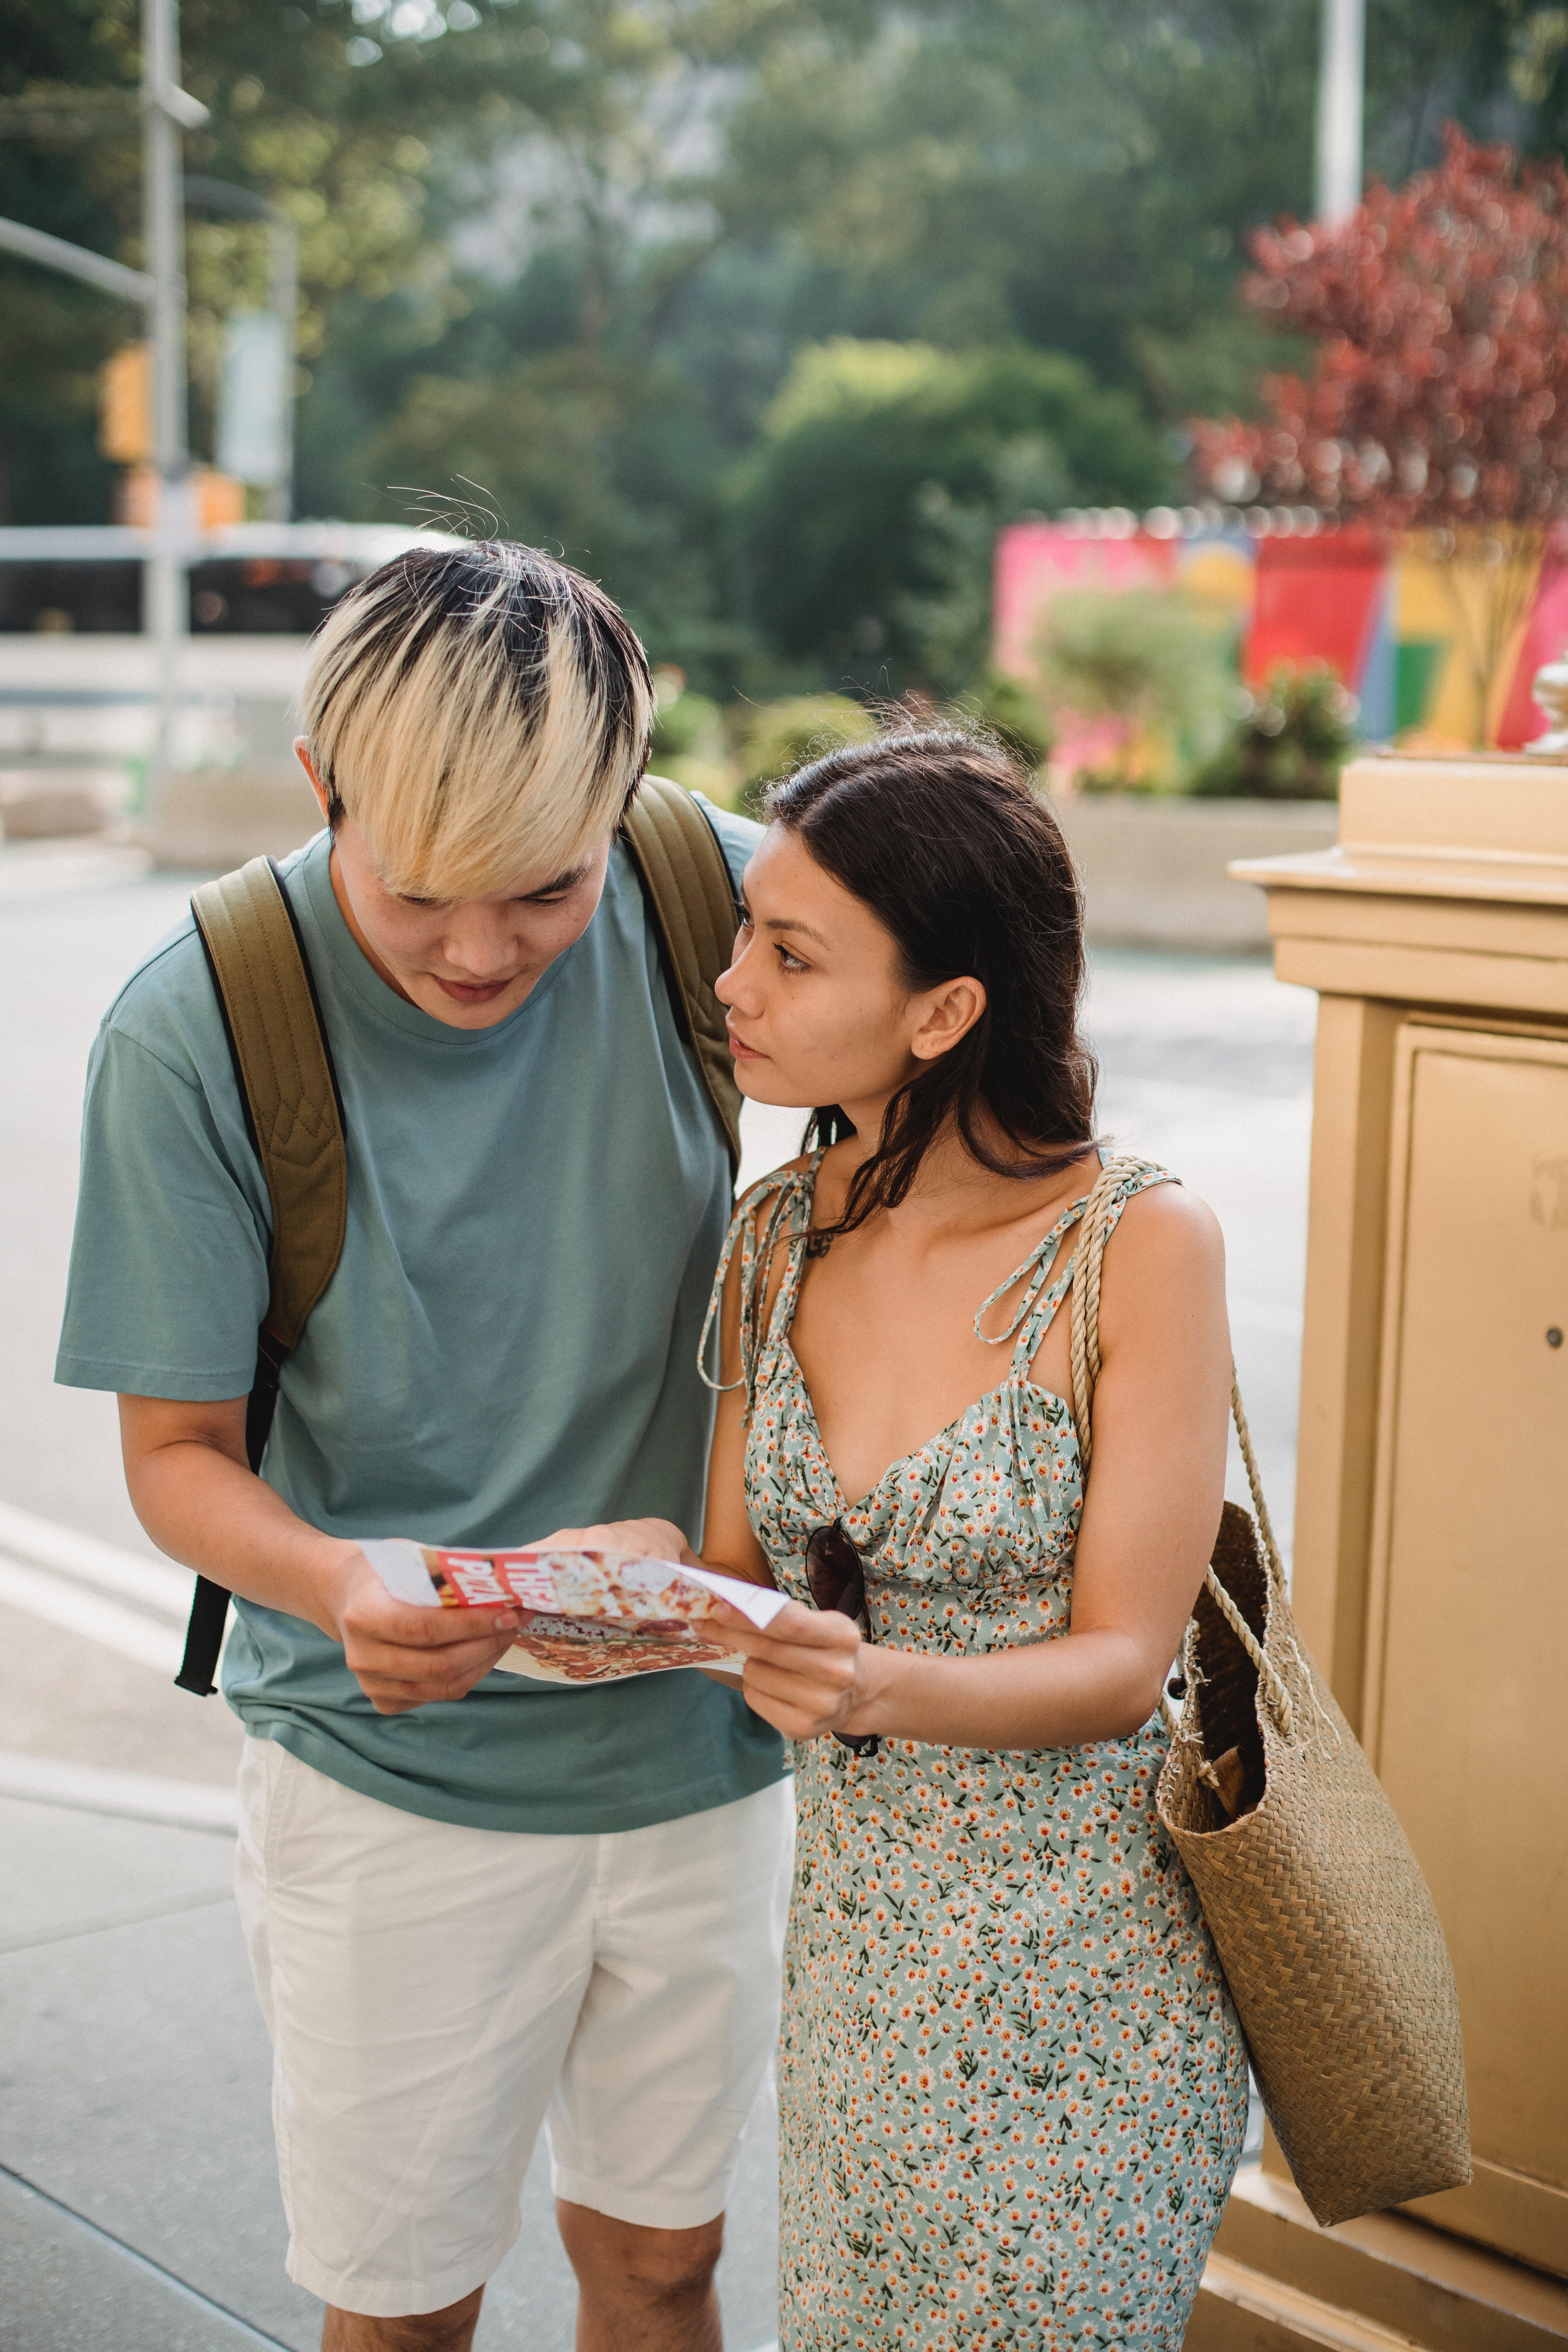
\includegraphics[width=0.5\textwidth]{media/no_gps.jpg}
		\caption{\url{https://www.pexels.com/de-de/foto/paar-das-route-in-der-karte-sucht-wahrend-sie-zusammen-reisen-5225256/}}
	\end{figure}
\end{columns}
\end{frame}

\begin{frame}
\begin{columns}
  \column{0.4\linewidth} 
	\begin{itemize}
		\item build an organizer 
		\item implement interaction possibilities
		\item find a way to offer event information offline (connectivity challenge)
	\end{itemize}
\column{0.6\linewidth}   
	 \begin{figure}
	 \centering
	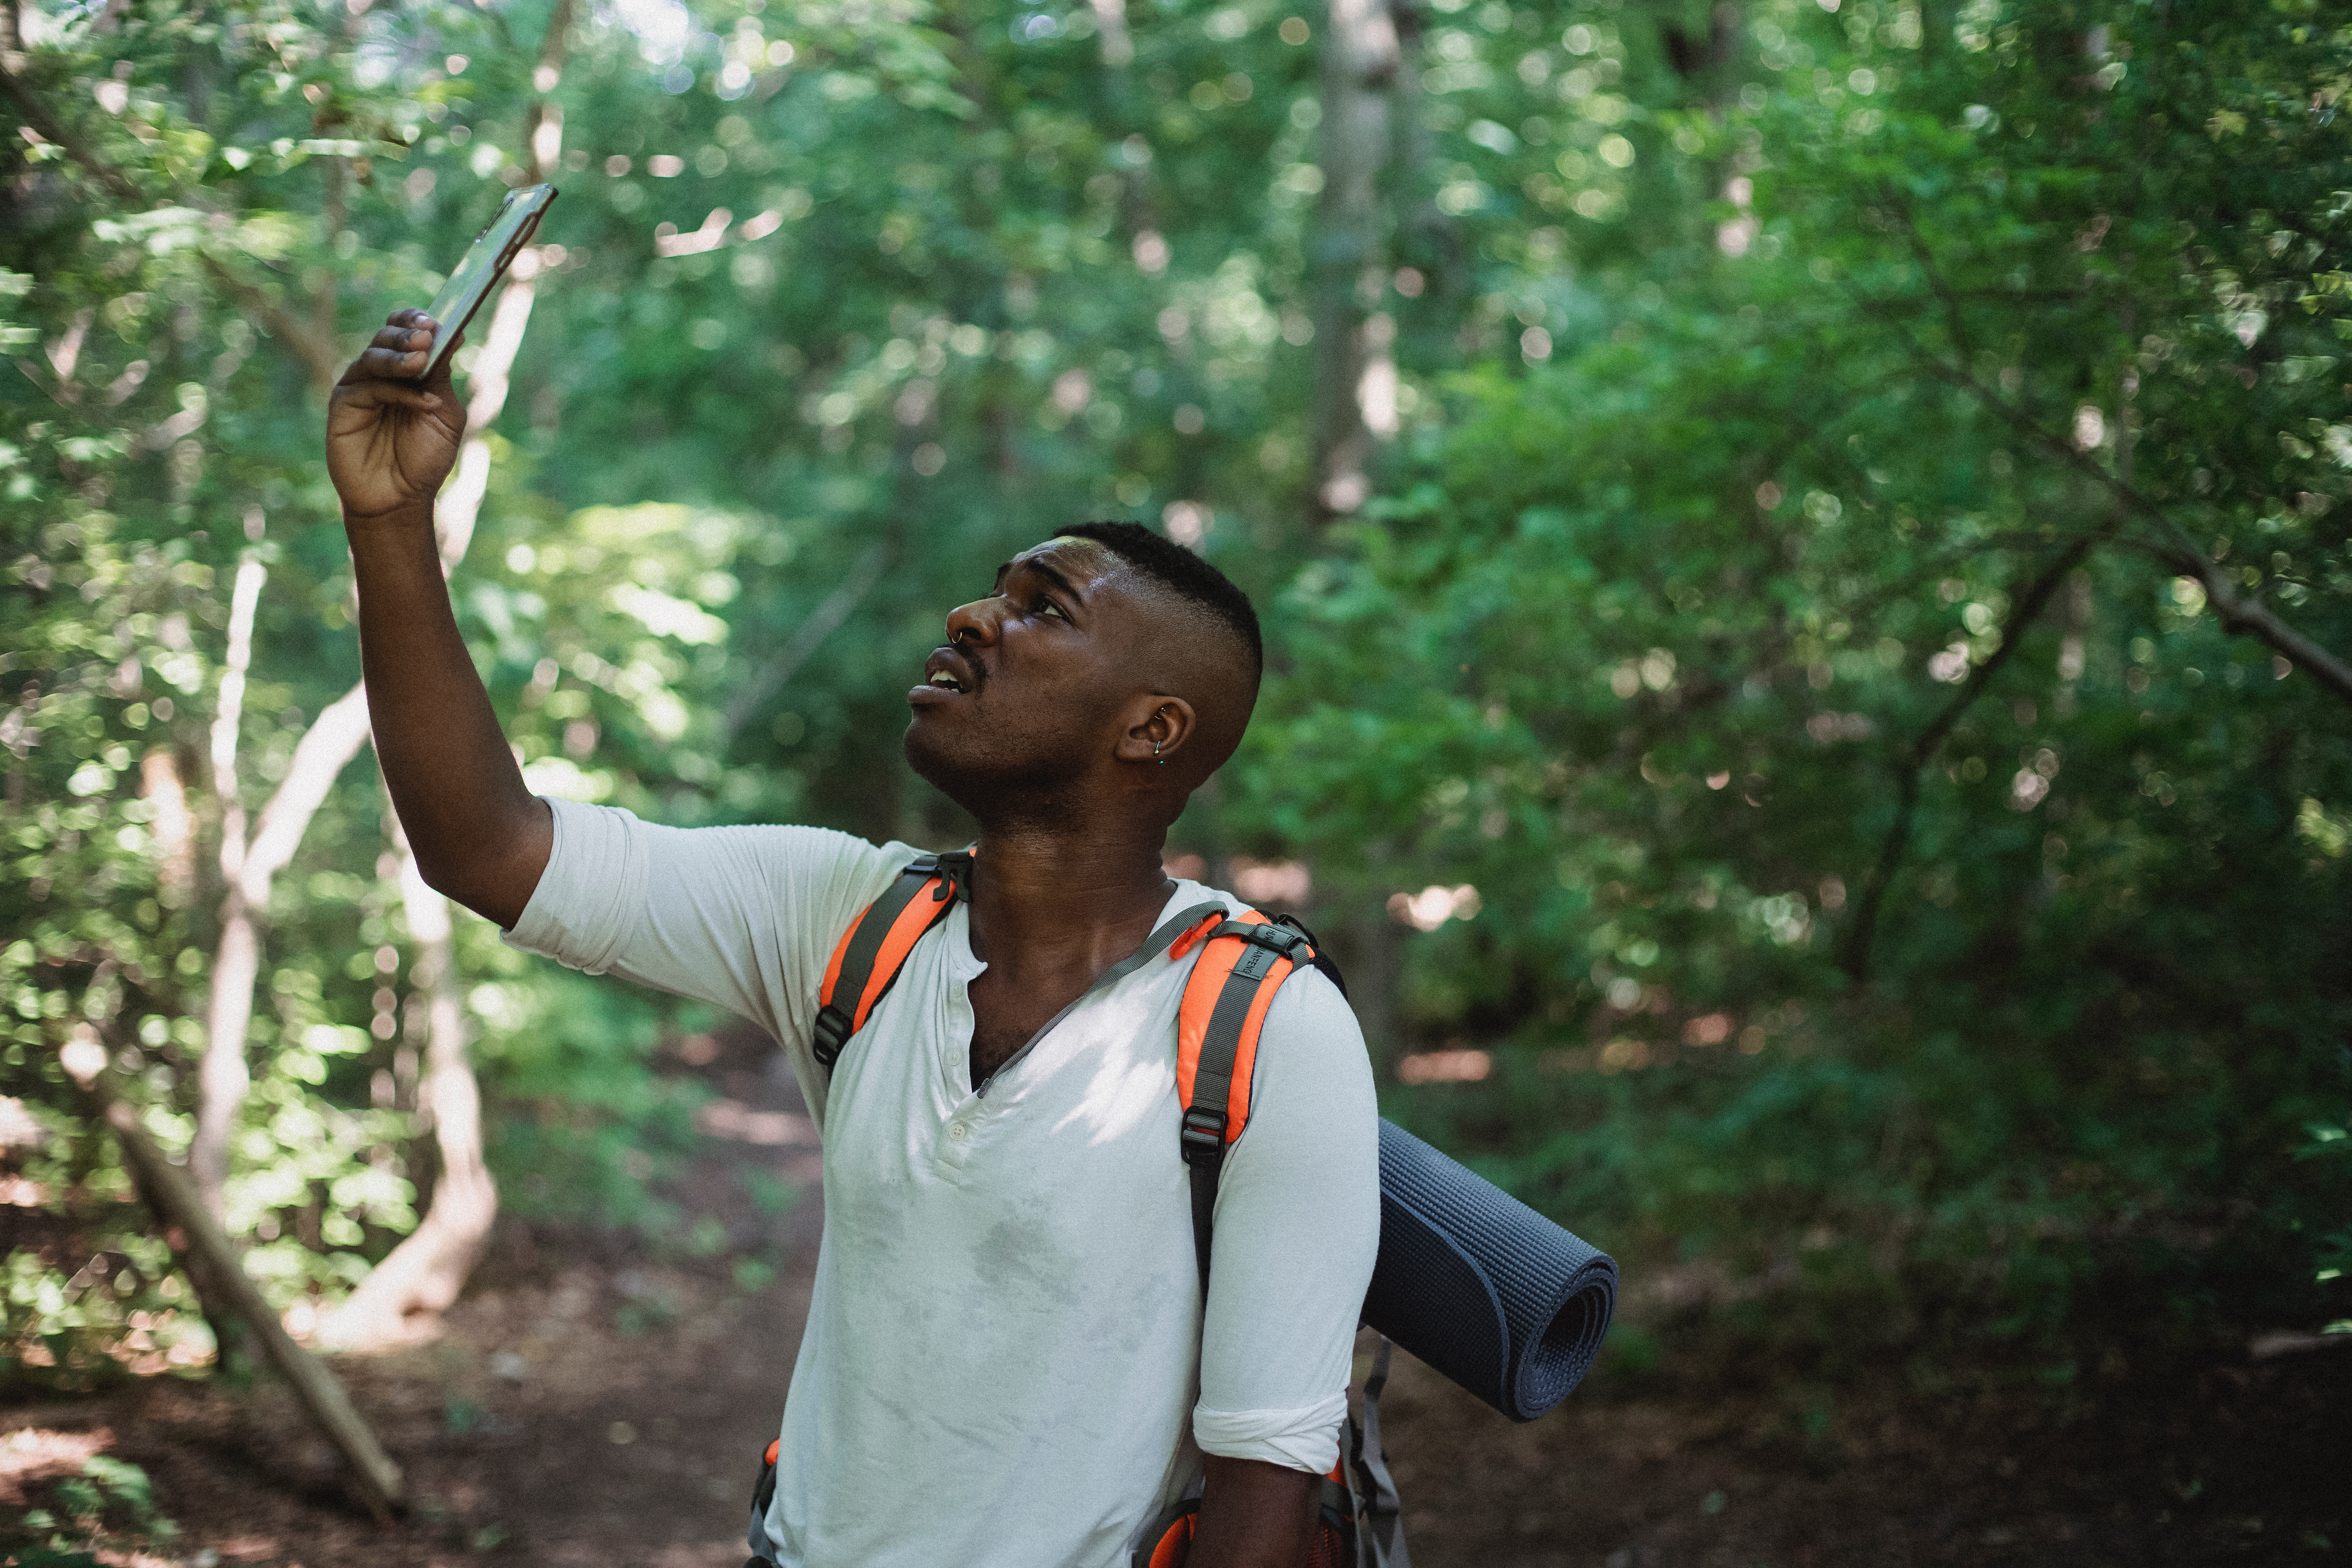
\includegraphics[width=1\textwidth]{media/no_internet.jpg}
	\caption{\url{https://www.pexels.com/de-de/foto/fokussierte-schwarze-reisende-die-verbindung-im-wald-sucht-5064614/}}
\end{figure}
\end{columns}
\end{frame}




\section{Architecture and key technologies}
\begin{frame}
\frametitle{Architecture}
We want to build our application using:
	\begin{itemize}
		\item a client-server model 
		\item the model-view-controller pattern
		\item a small, lightweight database
	\end{itemize}
\end{frame}

\begin{frame}
\frametitle{Key technologies}
	\begin{columns}
  \column{0.4\linewidth} 
used in our application:
  \begin{itemize}
		\item GPS Sensors 
		\item internet connection
		\item local storage
  \end{itemize}
  \column{0.4\linewidth}   
    used to build our application:
  \begin{itemize}
		\item Android Studio
		\item Java
		\item Web Server
  \end{itemize}
\end{columns}
\end{frame}

\end{document}